\section{Task IV : Key Events and Great Athletes}
\subsection{Key Events}
\subsubsection{Calculation Methods}
To identify key events, we will use the proportion of medals from these events among the whole medal tally as a main factor.

\begin{figure}[htbp]
    \centering
    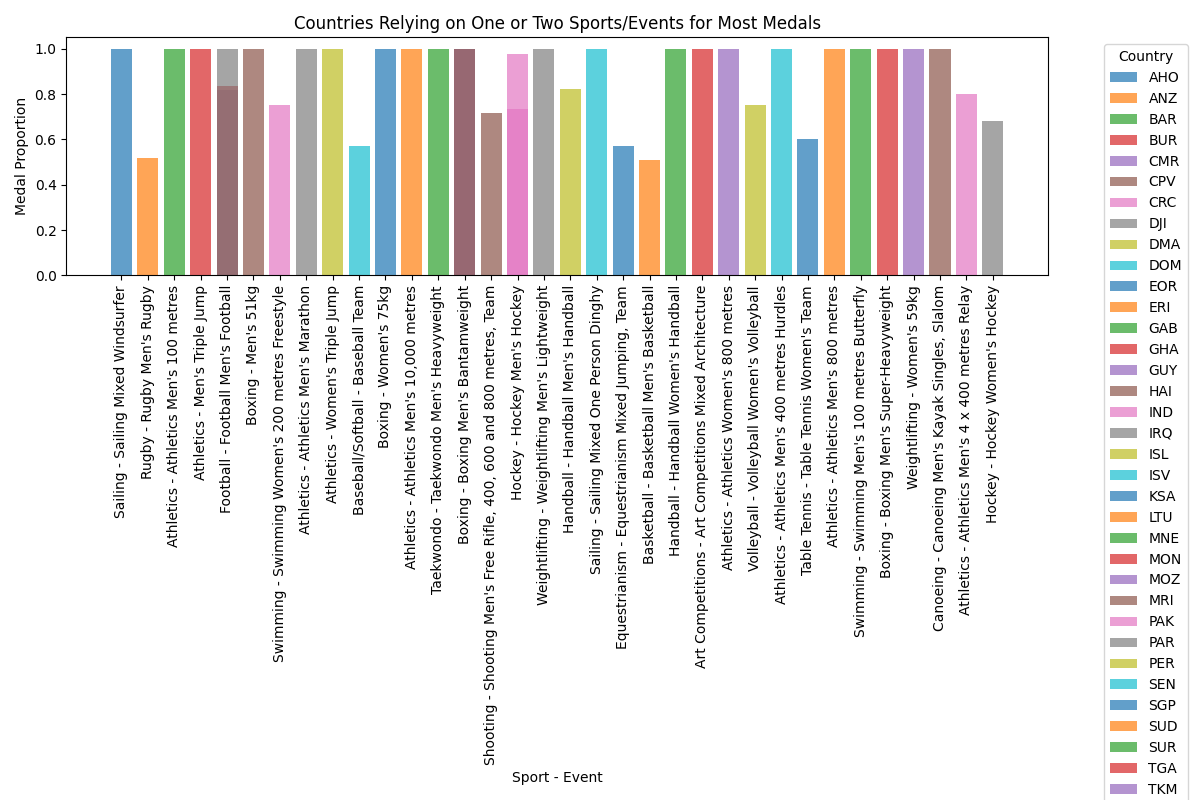
\includegraphics[width=1.1\textwidth]{./figures/Key_event.png}
    \caption{ Countries with biased medal distribution}
    \label{fig:Key_event}
\end{figure}

From this graph, we can see that many countries rely on one or two sports/events for their medal tally. This can be inspiring for the countries' Olympics committees.

\subsection{Great Athletes}
\subsubsection{Calculation Methods}
To identify Great Athletes, we would like to see those who secured almost all the (Gold) medals in their careers. Often, these Athletes play a significant role in their countries' Olympics team for
winning medals, or at least in this certain sport/event.

% \begin{figure}[htbp]
%     \centering
%     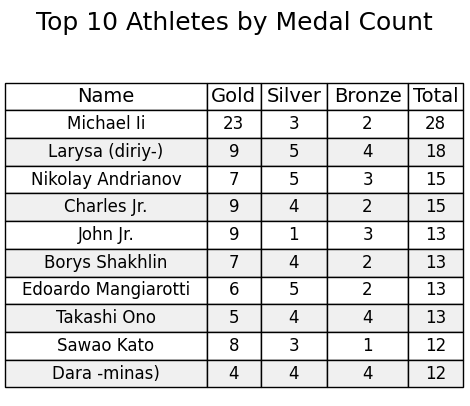
\includegraphics[width=0.8\textwidth]{./figures/Top10_Athlete.png}
%     \caption{ Countries with biased medal distribution}
%     \label{fig:Top10_Athlete}
% \end{figure}

From the graph we can see that \textbf{Great Athletes} can impact the event and their countries performance greatly, which can be also inspiring for the countries' Olympics committees,
for instance, how to cope with the possible downfall of the national team's performance after these great stars retired.
